\documentclass[12pt]{book}
\usepackage{tgschola}
\usepackage{longtable}
\usepackage{hyperref}
\usepackage[utf8]{inputenc}
\usepackage[margin=1in]{geometry}
\usepackage{tikz}
\usetikzlibrary{shapes.geometric, arrows, positioning}

\title{The Robot Plumbing Guide}
\date{\today}
\author{The Hibike Team}
\begin{document}
\maketitle

\tableofcontents

\chapter{Introduction}
The driving principle behind PiE is running a robotics competition. This means many things:
logistics, provinding mentorship and guidance, organizing events,
providing an interface for programming the robot, and making
the robot work. Keep in mind that this guide addresses only one aspect
of the competition; plumbing is not everything. With that said, it is still a good
idea to have a plumber on hand when pipes start to leak.
\section{A Brief Overview of the Control Stack}
For our purposes, there are four elements involved in controlling the robot.
\begin{enumerate}
	\item Dawn: the main interface that students use. Takes inputs from the controller,
	    and shows data and errors to students.
	\item Runtime: the program in charge of monitoring and communication. Sends and receives data from
        Dawn (via Ansible), as well as monitoring Hibike and StateManager.
	\item StateManager: a data store. Provides a central place to store and retrive data from Hibike
	    and Runtime.
	\item Hibike: the program that communicates with sensors. Handles low-level protocol details.
\end{enumerate}
\section{An Analogy}
A simple way to explain the role of each component in the stack, from Dawn to Hibike, is
as an analogy to a company.

Dawn is the CEO, the main person in charge. Every other system starts or stops
on her word, and follows her orders to the letter. Runtime is the middle manager. He
passes information from underlings on to the boss, relays her orders to them, and makes
sure that they are working. StateManager is the record-keeper. He stores information
that Hibike and Runtime give him, and retrieves it when they ask for it. Hibike is
in charge of a bunch of interns, the sensors. She asks them to periodically give her
updates on what they are doing, and fires them if they don't.
\section{A Diagram of the Stack}
\begin{center}
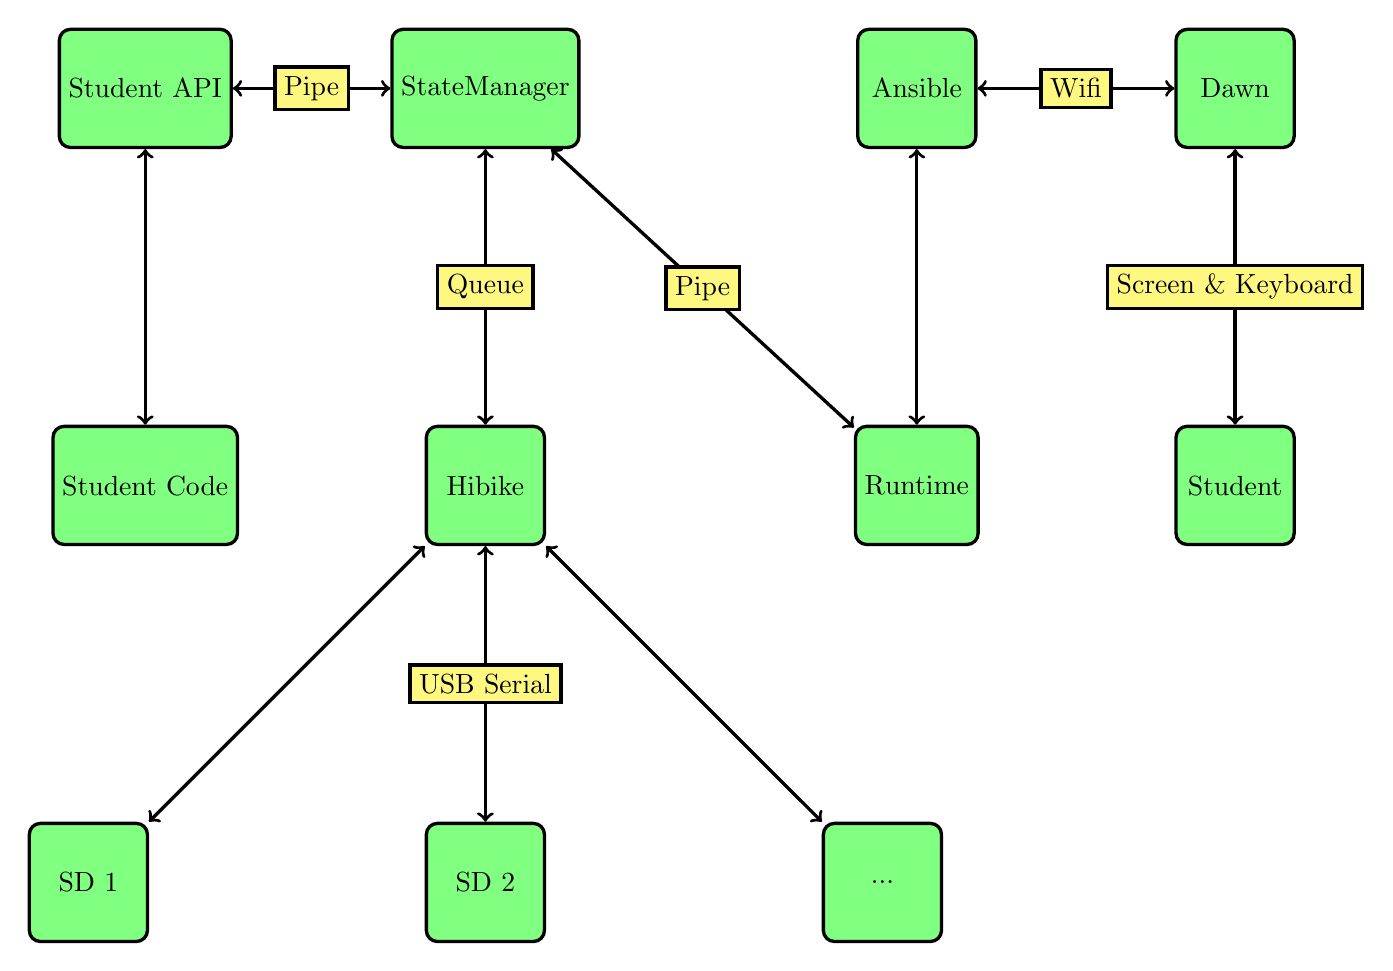
\begin{tikzpicture}[node distance=3.5cm, part/.style={
        rectangle,
        rounded corners,
        draw=black,
        text=black,
        fill=green!50,
        minimum size=1.5cm,
        very thick
    }, method/.style={
        rectangle,
        draw=black,
        fill=yellow!50,
    }, arrow/.style={
        very thick, <->, =>stealth
    }]
    \node (smgr) [part] {StateManager};
    \node (ansible) [part, right=of smgr] {Ansible};
    \node (dawn) [part, right=of ansible, xshift=-1cm] {Dawn};
    \node (student) [part, below=of dawn] {Student} ;
    \node (runtime) [part, below=of ansible] {Runtime};
    \node (hibike) [part, below=of smgr] {Hibike};
    \node (smrt1) [part, below=of hibike] {SD 2};
    \node (smrt2) [part, right=of smrt1] {...};
    \node (smrtmore) [part, left=of smrt1] {SD 1};
    \node (studentapi) [part, left=of smgr, xshift=1.5cm] {Student API};
    \node (studentcode) [part, below=of studentapi] {Student Code};
    \draw [arrow] (studentcode) -- (studentapi);
    \draw [arrow] (studentapi) -- node[method] {Pipe} (smgr);
    \draw [arrow] (runtime) -- (ansible);
    \draw [arrow] (student) -- node[method] {Screen \& Keyboard} (dawn);
    \draw [arrow] (dawn) -- node[method] {Wifi} (ansible);
    \draw [arrow] (smgr) -- node[method] {Pipe} (runtime);
    \draw [arrow] (smgr) -- node[method] {Queue} (hibike);
    \draw [arrow] (hibike) -- (smrt2);
    \draw [arrow] (hibike) -- node[method] {USB Serial} (smrt1);
    \draw [arrow] (hibike) -- (smrtmore);

\end{tikzpicture}
\end{center}
\chapter{Hibike}
Hibike is in charge of low-level sensor communication, and all the gory
details that are involved. It is divided into two modules:
\begin{itemize}
	\item \texttt{hibike\_message.py}

	The low-level details of the
	Hibike communications protocol. Handles things like encoding into packets and checksums.
	\item \texttt{hibike\_process.py}

	The ``supervisor'' of sensors.
	Communicates with sensors, sends data to runtime, and reacts to orders from StateManager.
\end{itemize}

Alongside these main modules, there are various testing modules:
\begin{itemize}
	\item \texttt{virtual\_device.py}

	Virtual devices, for testing Hibike's read and write capabilities.
	\item \texttt{hibike\_tester.py}

	A test module that wraps a Hibike process with a nicer interface.
\end{itemize}

\section{Design Choices and Explanations}
Hibike is packet-based and works over USB, specifically serial.

\paragraph{Why USB?}

In previous years, a custom communications protocol was used, over custom cables.
This provided the advantage of real-time and configurability; however, debugging was very difficult,
and developing for smart sensors more so. The Beaglebone doesn't provide real-time guarantees
anyways, and USB provides cheap, commodity cables and well-tested software.

\paragraph{Why packets?}

Most protocols are packet-based, and serial is not a packet-based communications link.
Packets make it easy to tell when data begins and ends.

\paragraph{Why serial?}

Arduino provides a well-tested serial library, so communication with any Arduino is easy
over serial. In addition, implementing and using serial is relatively simple compared
to many other types of USB connection, such as HID (used by keyboards and mice). Some
flexibility and speed is lost as a result of this abstraction, but much more is gained
in ease of use.

\section{The Hibike Protocol}
\subsection{A Quick Introduction}
We make a few starting assumptions concerning the endpoints of communication: the device controlling a sensor is a Smart Device (SD), and a Beaglebone Black (BBB) is used as the central control board of each robot and thus is in charge of communicating with each Smart Device. These two communicate with each other via serial: the Beaglebone running pySerial and the Smart Device by using the built-in serial library. As each Smart Device communicates with the Beaglebone on its own separate port, we conveniently have no need to worry about any race conditions or other problems arising from concurrency.

Hibike abstracts every Smart Device as a set of (parameter, value) pairs.
The hibike protocol supports three ways of interacting with these parameters:
\begin{itemize}
\item Subscribing to regular updates of specific paramters
\item Polling specific parameters
\item Writing to specific parameters
\end{itemize}

Refer to Section 7 for an outline of the general behavior of the Hibike protocol.

\subsection{Message Format}

All messages have the relatively simple structure of Message ID, Payload, and Checksum as
depicted below. A more complete description of each field is given below the diagram.

\begin{center}
	\begin{tabular}{|c|c|c|c|}
	\hline
	Message ID & Payload Length & Payload & Checksum \\
	(8 Bits) & (8 Bits) & (Length Varies) & (8 Bits) \\
	\hline
	\end{tabular}
\end{center}

\begin{itemize}
	\item Message ID
	\begin{itemize}
		\item An 8-bit ID specifying the type of message.
		\item More information about this field in the following sections.
	\end{itemize}
	\item Payload Length
	\begin{itemize}
		\item An 8-bit unsigned integer, specifying the number of bytes in the payload.
	\end{itemize}
	\item Payload
	\begin{itemize}
		\item Varies depending on the type of message sent.
	\end{itemize}
	\item Checksum
	\begin{itemize}
		\item An 8-bit checksum placed at the end of every message.]
		\item The current scheme XORs every other byte in the message.
	\end{itemize}
\end{itemize}

\subsection{UID Format}
Each smart device is assigned an 88-bit UID with the following fields.

\begin{center}
	\begin{tabular}{|c|c|c|}
	\hline
	Device Type & Year & ID \\
	(16 Bits) & (8 Bits) & (64 bits) \\
	\hline
	\end{tabular}
\end{center}

\begin{itemize}
	\item Device Type
	\begin{itemize}
		\item 16-bit ID specifying the Type of a Smart Device
		\item Device types are enumerated in Section 5
	\end{itemize}
	\item Year
	\begin{itemize}
		\item 8-bit ID corresponding to the competition year that the Smart Device was manufactured for.
		\item The 2015-2016 season will correspond to 0x00
	\end{itemize}
	\item ID
  	\begin{itemize}
  		\item Randomly generated 64-bit number that will uniquely identify each Smart Device within a specific device type and year.
  		\item With 64-bit IDs, the probability of a hash collision with 1000 of 1 type of device per year is roughly 0.05\%
	\end{itemize}
\end{itemize}

\subsection{Parameters and Bitmaps}

\begin{itemize}
	\item Hibike abstracts every smart device as a set of parameters that map to values
	\item Each smart device contains some number of paramaters, which can be read/written to.
	\item Parameters can have many types. The following types are supported:
	\begin{itemize}
		\item \texttt{bool}
		\item \texttt{uint8\_t}
		\item \texttt{int8\_t}
		\item \texttt{uint16\_t}
		\item \texttt{int16\_t}
		\item \texttt{uint32\_t}
		\item \texttt{int32\_t}
		\item \texttt{uint64\_t}
		\item \texttt{int64\_t}
		\item \texttt{float}
		\item \texttt{double}
	\end{itemize} CAUTION: Arduino's doubles are only 4 bytes long (same as a float), so an
	Arduino's Double is the same as python's Float. Do not use this type
	unless your arduino is actually cranking out 8 bytes.
	\item Some paramaters are read only, some are write only, and some support both.
	\item A config file will describe the paramaters for each Device Type (name, type, permissions).
	\item Some packets encode sets of parameters in the form of bitmaps.
	\begin{center}
		\begin{tabular}{|c|c |c| c|}
		\hline
		Params & Value 0 & \ldots & Value 15 \\
		(16 bits) & (Optional and Variable) & \ldots & (Optional and Variable) \\
		\hline
		\end{tabular}
	\end{center}
	\begin{itemize}
		\item Params - 16-bit bitmap describing a set of parameters. The nth bit of
		Params, where the LSB is the 0th bit, references the nth paramater of
  		a device.
		\item Value{[}0-15{]} - DeviceWrite and DeviceData send actual values for
  		each param in Params. The value field for param n will only be present
  		if bit n in Params is set. The size and type of each value field
  		depends on param number and device type, and is described in a config
  		file.
  	\end{itemize}
\end{itemize}

\subsection{Message Types}
\begin{center}
    \begin{tabular}{|c|c|}
        \hline
        ID & Message Type \\
        \hline
        0x10 & Ping \\
        0x11 & Subscription Request \\
        0x12 & Subscription Response \\
        0x13 & Device Read \\
        0x14 & Device Write \\
        0x15 & Device Data \\
        0x16 & Device Disable \\
        0x17 & Heartbeat Request \\
        0x18 & Heartbeat Response \\
        0xFF & Error \\
        \hline
    \end{tabular}
\end{center}

\subsection{Device Types}
% This part was automatically converted from the README
\begin{longtable}[c]{@{}|l|l|l|l|l|l|l|@{}}
\toprule
ID & Sensor & Param Number & Param Name & Param Type & Read? &
Write?\tabularnewline
\midrule
\endhead
\hline
0x00 & LimitSwitch & 0 & switch0 & bool & yes & no\tabularnewline
& & 1 & switch1 & bool & yes & no\tabularnewline
& & 2 & switch2 & bool & yes & no\tabularnewline
0x01 & LineFollower & 0 & left & float & yes & no\tabularnewline
& & 1 & center & float & yes & no\tabularnewline
& & 2 & right & float & yes & no\tabularnewline
0x02 & Potentiometer & 0 & pot0 & float & yes & no\tabularnewline
& & 1 & pot1 & float & yes & no\tabularnewline
& & 2 & pot2 & float & yes & no\tabularnewline
0x03 & Encoder & 0 & rotation & int16\_t & yes & no\tabularnewline
0x04 & BatteryBuzzer & 0 & is\_unsafe & bool & yes & no\tabularnewline
& & 1 & calibrated & bool & yes & no\tabularnewline
& & 2 & v\_cell1 & float & yes & no\tabularnewline
& & 3 & v\_cell2 & float & yes & no\tabularnewline
& & 4 & v\_cell3 & float & yes & no\tabularnewline
& & 5 & v\_batt & float & yes & no\tabularnewline
& & 6 & dv\_cell2 & float & yes & no\tabularnewline
& & 7 & dv\_cell3 & float & yes & no\tabularnewline
0x05 & TeamFlag & 0 & mode & bool & yes & yes\tabularnewline
& & 1 & blue & bool & yes & yes\tabularnewline
& & 2 & yellow & bool & yes & yes\tabularnewline
& & 3 & led1 & bool & yes & yes\tabularnewline
& & 4 & led2 & bool & yes & yes\tabularnewline
& & 5 & led3 & bool & yes & yes\tabularnewline
& & 6 & led4 & bool & yes & yes\tabularnewline
0x06 & Grizzly & & & & &\tabularnewline
0x07 & ServoControl & 0 & servo0 & float & yes & yes\tabularnewline
& & 1 & servo1 & float & yes & yes\tabularnewline
0x08 & LinearActuator & & & & &\tabularnewline
0x09 & ColorSensor & & & & &\tabularnewline
0x0A & YogiBear & 0 & duty\_cycle & float & yes & yes\tabularnewline
& & 1 & pid\_pos\_setpoint & float & no & yes\tabularnewline
& & 2 & pid\_pos\_kp & float & no & yes\tabularnewline
& & 3 & pid\_pos\_ki & float & no & yes\tabularnewline
& & 4 & pid\_pos\_kd & float & no & yes\tabularnewline
& & 5 & pid\_vel\_setpoint & float & no & yes\tabularnewline
& & 6 & pid\_vel\_kp & float & no & yes\tabularnewline
& & 7 & pid\_vel\_ki & float & no & yes\tabularnewline
& & 8 & pid\_vel\_kd & float & no & yes\tabularnewline
& & 9 & current\_thresh & float & no & yes\tabularnewline
& & 10 & enc\_pos & float & yes & yes\tabularnewline
& & 11 & enc\_vel & float & yes & no\tabularnewline
& & 12 & motor\_current & float & yes & no\tabularnewline
& & 13 & deadband & float & yes & yes\tabularnewline
0x0B & RFID & 0 & id & uint8\_t & yes & no\tabularnewline
& & 1 & detect\_tag & uint8\_t & yes & no\tabularnewline
0x10 & DistanceSensor & & & & &\tabularnewline
0x11 & MetalDetector & & & & &\tabularnewline
0xFFFF & ExampleDevice & 0 & kumiko & bool & yes & yes\tabularnewline
& & 1 & hazuki & uint8\_t & yes & yes\tabularnewline
& & 2 & sapphire & int8\_t & yes & yes\tabularnewline
& & 3 & reina & uint16\_t & yes & yes\tabularnewline
& & 4 & asuka & int16\_t & yes & yes\tabularnewline
& & 5 & haruka & uint32\_t & yes & yes\tabularnewline
& & 6 & kaori & int32\_t & yes & yes\tabularnewline
& & 7 & natsuki & uint64\_t & yes & yes\tabularnewline
& & 8 & yuko & int64\_t & yes & yes\tabularnewline
& & 9 & mizore & float & yes & yes\tabularnewline
& & 10 & nozomi & double & yes & yes\tabularnewline
& & 11 & shuichi & uint8\_t & yes & no\tabularnewline
& & 12 & takuya & uint16\_t & no & yes\tabularnewline
& & 13 & riko & uint32\_t & yes & no\tabularnewline
& & 14 & aoi & uint64\_t & no & yes\tabularnewline
& & 15 & noboru & float & yes & no\tabularnewline
\bottomrule
\end{longtable}

\subsection{Error Types}
\begin{tabular}{|c|c|}
    \hline
    Status & Meaning \\
    \hline
    0xFD & Unexpected Packet Delimiter \\
    0xFE & Checksum Error \\
    0xFF & Generic Error \\
    \hline
\end{tabular}

\subsection{Message Descriptions}
\begin{enumerate}
    \item Ping: BBB pings SD for enumeration purposes.
        The SD will respond with a SubscriptionResponse packet.
        
        Payload format:
        \begin{center}
            \begin{tabular}{|c|c|}
                \hline
                Empty \\
                (0 bits) \\
                \hline
            \end{tabular}
        \end{center}
        Direction: BBB $\Rightarrow$ SD

    \item SubscriptionRequest: BBB requests data to be returned at a given interval.
        \begin{itemize}
            \item Params is a bitmap of paramaters being subscribed to.
            \item The SD will respond with a Sub Response packet with a delay and
                bitmap of params it will acutally send values for, which may not be
                what was requested, due to nonexistent and write-only parameters.
            \item If too many parameters are subscribed to, the Smart Device may have
                to send multiple DeviceData packets at each interval.
            \item A delay of 0 indicates that the BBB does not want to receive data.
            \item Non-zero delay with 0 Params will still subscribe to empty
                updates!!!
        \end{itemize}
        Payload format:
        \begin{center}
            \begin{tabular}{|c|c|}
                \hline
                Params & Delay \\
                (16 bits) & (16 bits) \\
                \hline
            \end{tabular}
        \end{center}
        Direction: BBB $\Rightarrow$ SD
    \item SubscriptionResponse: SD sends (essentially) an ACK packet with its UID,
        params subscribed to, and delay.

        Payload format:
        \begin{center}
            \begin{tabular}{|c|c|c|}
                \hline
                Params & Delay & UID \\
                (16 bits) & (16 bits) & (88 bits) \\
                \hline
            \end{tabular}
        \end{center}
        Direction: BBB $\Leftarrow$ SD
    \item Device Read: BBB requests some values from the SD.
        \begin{itemize}
            \item The SD should respond with DeviceData packets with values for all
                the readable params that were requested.
            \item If all the values cannot fit in one packet, multiple will be sent.
        \end{itemize}

        Payload format:
        \begin{center}
            \begin{tabular}{|c|}
                \hline
                Params \\
                (16 bits) \\
                \hline
            \end{tabular}
        \end{center}
        Direction: BBB $\Rightarrow$ SD
    \item Device Write: BBB writes attempts to write values to some parameters.
        \begin{itemize}
            \item The SD should respond with a DeviceData packet describing the
                readable params that were actually written to.
            \item The protocol currently does not support any ACK for write only
                params.
        \end{itemize}

        Payload format:
        \begin{center}
            \begin{tabular}{|c|c|c|c|}
                \hline
                Params & Value 0 & \ldots & Value 15 \\
                (16 bits) & (Optional and Variable) & \ldots & (Optional and Variable) \\
                \hline
            \end{tabular}
        \end{center}
        Direction: BBB $\Rightarrow$ SD
    \item Device Data: SD sends the values of some of its paramters.
        \begin{itemize}
            \item This can occur in response to a DeviceWrite/DeviceRead, or when the
                interval for a SubscriptionResponse occurs.
        \end{itemize}
        Payload format:
        \begin{center}
            \begin{tabular}{|c|c|c|c|}
                \hline
                Params & Value 0 & \ldots & Value 15 \\
                (16 bits) & (Optional and Variable) & \ldots & (Optional and Variable) \\
                \hline
            \end{tabular}
        \end{center}

        Direction: BBB $\Leftarrow$ SD
    \item Heart Beat Request: BBB/SD requests SD/BBB heartbeat response for
        connectivity purposes.
        \begin{itemize}
            \item This message pathway is a two way street, both BBB and SD can send
                requests and send responses to the other
            \item Upon receiving a Heart Beat Request, a Heart Beat Response message
                should be immediately sent back
            \item Payload is currently unused, but can be used for future
                functionality in keeping track of individual heartbeat requests and
                responses (for latency purposes)
        \end{itemize}
        Payload format:
        \begin{center}
            \begin{tabular}{|c|}
                \hline
                ID \\
                (8 bits) \\
                \hline
            \end{tabular}
        \end{center}
        Direction: BBB $\Leftrightarrow$ SD
    \item Heart Beat Response: Sent in response to a Heart Beat Request
        \begin{itemize}
            \item This message pathway is a two way street, both BBB and SD can
                receive requests and send responses to the other
            \item Should only be sent upon receiving a Heart Beat Request
            \item Payload is currently unused, but can be used for future
                functionality in keeping track of individual heartbeat requests and
                responses (for latency purposes)
        \end{itemize}
        Payload format:
        \begin{center}
            \begin{tabular}{|c|}
                \hline
                ID \\
                (8 bits) \\
                \hline
            \end{tabular}
        \end{center}
        Direction: BBB $\Leftrightarrow$ SD
    \item Error Packet: Sent to indicate an error occured.
        \begin{itemize}
            \item Currently only used for the BBB to log statistics.
        \end{itemize}
        Payload format:
        \begin{center}
            \begin{tabular}{|c|}
                \hline
                Error Code\\
                (8 bits) \\
                \hline
            \end{tabular}
        \end{center}
        Direction: BBB $\Leftarrow$ SD

\end{enumerate}

\section{The Hibike Process}
\texttt{hibike\_process.py} handles communication with sensors and StateManager.
Initialization and running happen in this series of steps:
\begin{enumerate}
    \item Hibike asks the operating system for a list of serial ports that match
        those used by Arduinos.
    \item It verifies that these ports are working, and opens them for communication.
    \item Hibike checks that each port contains a smart sensor by pinging it.
    \item Each device is given a reading thread, a writing thread, and a write queue.
    \item Alongside the device threads, a read batching thread and a cleanup
        thread are started. The batch thread sends all reads to StateManager
        at certain intervals. The cleanup thread removes disconnected devices.
    \item Hibike tells all devices to stop sending data. Once the devices
        respond, StateManager subscribes to each device for each of
        its parameters.
    \item Afterwards, Hibike receives and reacts to commands from StateManager.
\end{enumerate}

\subsection{An Explanation of the Architecture}
Each part of the structure of the Hibike process has its place, and has
been designed in deliberately. If threads are used, it is usually because
of blocking I/O.

\paragraph{Reader and Writer Threads}
Reading from a serial connection using nonblocking communication means that it
is easily possible to receive an incomplete packet even if the communications
link is reliable; thus, we use blocking reads. We don't want to stop reading
from every other sensor if one is taking a while, so we use threads to
periodically switch between sensors.

\paragraph{The Write Queue}
If a device sends a heartbeat request, we want to respond quickly
without going all the way to StateManager. Thus, we have a write queue, allowing
both the main thread and the read thread to write packets.

\paragraph{The Batch Thread}
Inter-thread communication is quick, but inter-process communication is slow.
Consequentially,
Hibike threads can quickly talk to each other, but talking to StateManager, which
runs in a separate process, is quite time-consuming. Instead of
sending any device data as soon as it is read, it is easier to bundle many
reads up and send them all at once. The batch thread is responsible for this.

\paragraph{The Cleanup Thread}
When a device disconnects, its resources remain in use. The read
and write threads sit idle, and the serial port remains open. This
can cause problems if a new device appears on an existing serial port,
so it is useful to clean up the resources. At the same time, it
can take up to 30 seconds to close a serial port, which is unacceptably
long for Hibike to wait. Therefore, a separate thread is put in charge
of such things.

\paragraph{The Hotplug Thread}
In order to detect new devices, something has to scan serial ports
and check which contain smart sensors. This could be done in the
main loop, but detection can take hundreds or even thousands of
milliseconds.

\section{Smart Devices}
There are a few types of smart device, each with its own responsibility.
Smart devices are based on the Arduino platform; we are using
Arduino Pro Micros because of their relative cheapness (\$4/unit)
and power. The firmware for these devices is written in C++.

\begin{itemize}
    \item LimitSwitch
        
        The name of this sensor is pretty self-explanatory. It's a limit
        switch (or two, or three), that is on when pressed.
    \item LineFollower

        This is a line-following sensor, that detects the brightness of
        the floor beneath it. There are three sensors: left, middle,
        and right.
    \item BatteryBuzzer

        This device monitors the battery voltage and cell balances,
        making sure that the battery doesn't get dangerously
        imbalanced or low. It displays the cell voltages
        on an LED display, and beeps when there are problems.
        Its functionality may be supplanted in
        the future by a dedicated chip.
    \item ServoControl

        The servo controller controls the position of a servo,
        in the range [-1, 1]. The position can be read or written to.

    \item YogiBear

        This is the new motor controller, put into place after the
        repeated demise of many a Grizzly. It uses a COTS motor controller,
        and has the ability to perform PID (supposedly). If Hibike
        does not respond to heartbeats, it disables itself automatically.

    \item RFID

        This sensor is unfortunately slow; sometimes, it will not read,
        and the read must be delayed for a cycle. It is also very close
        range; usually, about 0.5in is the maximum.
\end{itemize}

\section{Hotplug}
Smart sensor hotplug has been a highly requested feature for some time now.
There are two halves to hotplug: adding new devices, and disconnecting old ones.
Both sides of the implementation are based on polling -- periodically checking
whether new devices have been connected, or old ones removed.

\subsection{Adding New Devices}
Every period of \texttt{HOTPLUG\_POLL\_INTERVAL} seconds, the hotplug thread
wakes up and goes looking for new devices. It does this using the existing
\texttt{get\_working\_serial\_ports}, excluding any ports that are already
attached to existing devices. Afterwards, it scans these serial ports for smart
sensors, and adds them to the list of devices, spinning up threads and queues
as appropriate.

\subsection{Removing Disconnected Devices}
After adding any new devices, we go on the lookout for old devices that
have been disconnected. When a device is disconnected, its read and
write threads crash, and we receive a message in \texttt{error\_queue}.
If we have only received one message from a device, we assume that the device may only
have been temporarily disconnected, and resend the message for the next iteration.
If the existing device has a different serial port, then we assume
that the device has reconnected.
Otherwise, we tell the cleanup thread to clean the device.

\section{Testing}
Hibike provides a few options for testing protocol compatibility
and generating data.
As of now, there is no option to test timing statistics except
manual probing with an oscilloscope. Work is being done to
construct a hardware testing rig, but it is not yet complete.

Always test your pull requests on \textit{real hardware} before
attempting to merge! There are not any Travis tests yet.
\subsection{\texttt{hibike\_tester.py}}
This module acts as a fake StateManager, spawning its own
copy of \texttt{hibike\_process}. You can use this to verify
that Hibike is sending device data to state manager, and that
it reacts appropriately to commands sent to it.
\subsection{\texttt{virtual\_device.py}}
This implements virtual devices, which communicate with Hibike
through a virtual serial port. It is meant to be used with
\texttt{spawn\_virtual\_device.py} to create virtual devices
and send data on them. It can be used to test Hibike's ability to
respond to devices.
\subsection{Unit Tests}
There are none yet, but you're welcome to add some.


\chapter{Runtime and StateManager}
\section{Runtime's Architecture}
Runtime supervises other processes and handles errors as they occur. It is
essentially a state machine that reacts to messages from Dawn and student
code. If any process crashes, Runtime would (ideally) be able to restart
it seamlessly, although this doesn't happen yet.

\paragraph{Why Pipes over Queues?}

A pipe is more limited than a queue in every respect; it is single-consumer,
single-producer, as opposed to multi-producer, multi-consumer.
However, what it lacks in flexibility, it makes up for in speed.
There is a noticeable difference when using pipes versus queues.
In a scenario where the flexibility is unnecessary, pipes win.

\subsection{Runtime Steps}
\begin{enumerate}
    \item Spawn StateManager, Hibike, and UdpReceiver.
    \item Run the state machine.
        \begin{enumerate}
            \item Check if E-Stop was triggered.
            \item Check if we have restarted too many times.
            \item React to things in the bad things queue.
        \end{enumerate}
\end{enumerate}
\section{StateManager}
StateManager is, in essence, a large key-value store. It is used as
a centralized place to store state for each process on the robot,
and, indirectly, as a way to communicate between processes.

\subsection{Architecture}
StateManager consists of a large number of methods and a few message queues/pipes.
It receives messages from Hibike, Runtime, and Student Code, and invokes
one of its functions based on who sent the message, and which message
was received. Each message type is enumerated in an Enum, located in
\texttt{runtimeUtil.py}. Every time a key is added to storage,
a timestamp is stored, although this functionality isn't used for anything.

\section{Ansible}
\subsection{Introduction and Overview}\label{introduction-and-overview}

This page will detail how Runtime communicates with Dawn. The code is
contained primarily in \texttt{Ansible.py}, with relative protos stored
in
\href{https://github.com/pioneers/PieCentral/tree/master/ansible-protos}{ansible-protos}.

There are two forms of communication with Dawn: UDP and TCP. UDP is used
for constant data transfer where it is not critical to not lose packets.
TCP is used to send data where it is critical to not lose information.
Communication with Dawn happens in three processes, which are spawned by
\texttt{runtime.py}. These three processes are \texttt{UDPSendClass},
\texttt{UDPRecvCLass}, \texttt{TCPClass}. \texttt{UDPSendClass} spawns
two threads, one for packaging and one for sending.
\texttt{UDPRecvClass} does not spawn threads, and receives and
unpackages in succession. \texttt{TCPClass} spawns two threads, one for
sending and one for receiving.

See \href{https://github.com/pioneers/PieCentral/wiki/Dawn-Runtime-Network-Protocol}{Dawn Runtime Network Protocol}
for specific networking details, and
\href{https://developers.google.com/protocol-buffers/docs/pythontutorial}{Google
Protobuf} for information on how to use protobufs in python.

\subsection{Starting the Processes}\label{starting-the-processes}

All processes are started by \texttt{runtime.py} via the
\texttt{spawn\_process} function. Initially, on startup, only the
\texttt{UDPRecvClass} class is spawned. This is because runtime needs to
learn the IP of Dawn, and can only do so after receiving one packet.
After determining the IP of Dawn and it is stored into
\texttt{StateManager}, \texttt{BAD\_EVENTS.NEW\_IP} is triggered which
now spawns \texttt{UDPSendClass} and \texttt{TCPClass}. Only one Dawn
instance can be connected at a time. Whenever Dawn disconnects,
\texttt{BAD\_EVENTS.DAWN\_DISCONNECTED} is triggered which terminates
all the processes and then respawns just \texttt{UDPRecvClass}. This is
the same as the initial state, and it repeats the entire process.

\subsection{UDPRecvClass}\label{udprecvclass}

This class runs as a single process. It receives the robot state
(\texttt{IDLE}, \texttt{AUTONOMOUS}, \texttt{TEELEOP}, \texttt{ESTOP}),
the team color, and gamepad data.. If there doesn't currently exist an
IP stored (this is the first time receiving from Dawn), the IP will also
be saved and the other two communication processes will be spun up. If
the received state is different from the current state, a command will
be sent to \texttt{StateManager.py} via the \texttt{BadThingsQueue} to
switch student code state. If the team flag color has not been set, a
command (\texttt{SM\_COMMANDS.SET\_TEAM}) will be sent to
\texttt{StateManager.py} to set the team flag to the appropriate color.
Then, it takes the unpackaged data containing the gamepad data, and
sends it to \texttt{StateManager.py}.

\subsection{UDPSendClass}\label{udpsendclass}

This class runs as two threads in a single process. One process
constantly receives data from \texttt{StateManager}, and packages up via
protobufs all the sensor information, and the current robot state. It
then stores the data into a\\
\texttt{TwoBuffer} object which is shared by both processes. The second
process takes the packaged data from the \texttt{TwoBuffer}, and sends
it to Dawn viw UDP.

\subsection{TCPClass}\label{tcpclass}

This class runs as two threads in a single process, one to send and one
to receive. Both use the same TCP connection. The sender sends console
logs to Dawn, as well as acknowledges that runtime is ready for student
code upload. The receiver receives the command that student code is
going to be uploaded. Furthermore, when the TCP connection is broken (as
caught by an \texttt{except}), this indicates that Dawn has disconnected
and \texttt{Ansible} state is reset to idle.

\section{Student Code/Student API}
Student code itself runs in a separate process isolated from runtime, so that
it is not possible to deadlock runtime from student code. In addition,
signal handlers are installed to ensure that the code will stop
working if stalled for too long. The API communicates with StateManager
through a pipe.

\section{Testing}
Currently, Runtime's tests are located in \texttt{studentCode.py}. What
exists now is pretty basic, consisting mainly of fetching from and
storing into StateManager.
\end{document}
